% !TeX root = ../main.tex
% Add the above to each chapter to make compiling the PDF easier in some editors.

\chapter{Results and Analysis}\label{chapter:results and analysis}
\section{Model Performance Analysis}

\subsection{Comparison with Benchmark Models}

In this section, we compare the performance of our Gaussian Process Regression (GPR) models with a benchmark model, specifically the Autoregressive Integrated Moving Average (ARIMA) model. The comparison is based on the Mean Squared Error (MSE) of predictions over different forecast horizons.

\begin{itemize}
    \item \textbf{ARIMA Model}: A traditional time series forecasting model that uses past values and past errors to predict future values.
    \item \textbf{Market Efficiency}: Assumes that markets are efficient and all investors have access to the same information.
    \item \textbf{Normal Distribution of Asset Returns}: Assumes that asset returns are normally distributed and can be described by their mean (expected return) and variance (risk).
\end{itemize}

\paragraph{Comparison with ARIMA}

We evaluated the predictive performance of the GPR and ARIMA models over different forecast horizons (5, 10, 13, 20, and 26 days). The Mean Squared Error (MSE) was used as the evaluation metric. The results are summarized in Table~\ref{tab:mse_comparison}.

\begin{table}[htbp]
\centering
\caption{Mean Squared Error (MSE) Comparison between GPR and ARIMA Models}
\label{tab:mse_comparison}
\begin{tabular}{cccc}
\toprule
\textbf{Forecast Horizon (Days)} & \textbf{ARIMA MSE} & \textbf{GPR MSE} & \textbf{Best Model} \\
\midrule
5  & 34.8847 & 15.8594 & GPR \\
10 & 45.7229 & 39.1529 & GPR \\
13 & 47.0780 & 58.2299 & ARIMA \\
20 & 78.4795 & 98.9632 & ARIMA \\
26 & 267.8519 & 195.5078 & GPR \\
\bottomrule
\end{tabular}
\end{table}

As shown in Table~\ref{tab:mse_comparison}, the GPR model outperforms the ARIMA model for shorter forecast horizons (5 and 10 days), exhibiting lower MSE values. However, for medium forecast horizons (13 and 20 days), the ARIMA model shows better performance. For the longest horizon (26 days), the GPR model again demonstrates a lower MSE compared to ARIMA.

\paragraph{Visual Comparison}

Figure~\ref{fig:prediction_comparison} illustrates the predicted values from both GPR and ARIMA models against the actual values over the forecast horizons.

\begin{figure}[h!]
\centering
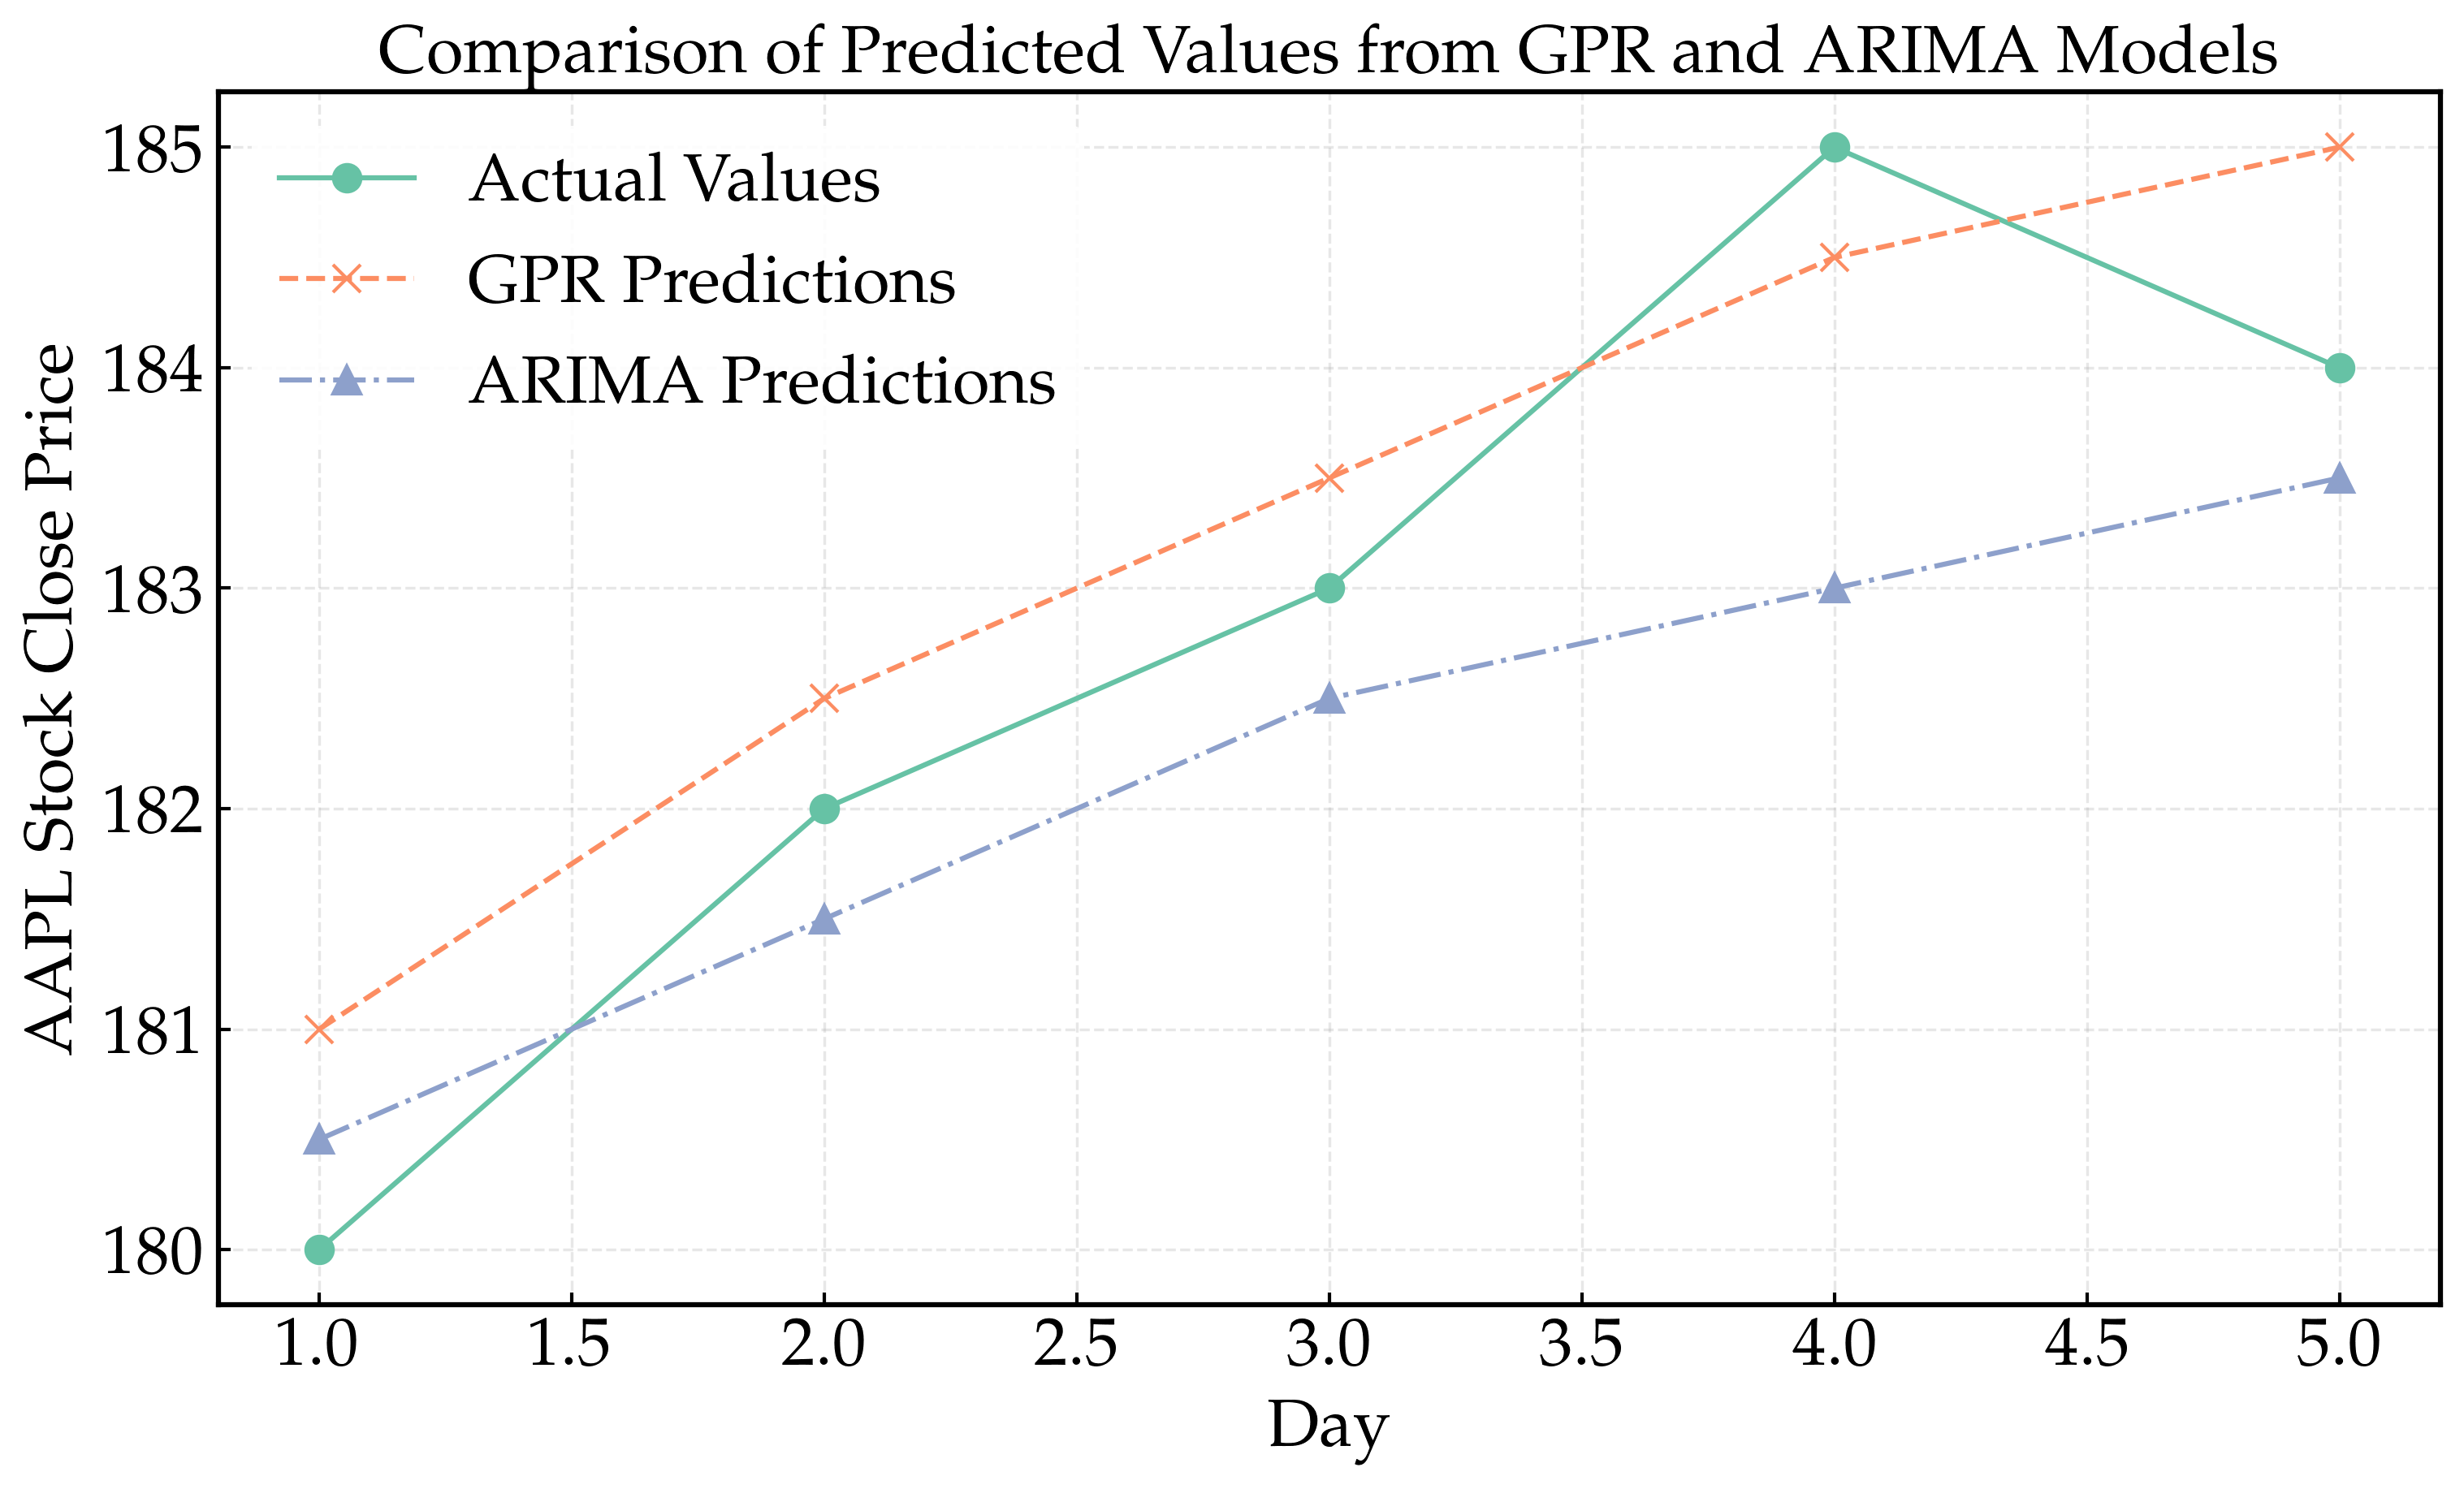
\includegraphics[width=0.8\textwidth]{prediction_comparison.png}
\caption{Comparison of Predicted Values from GPR and ARIMA Models}
\label{fig:prediction_comparison}
\end{figure}

\noindent In the figure, the actual values are plotted alongside the predictions from both models. The visual comparison allows us to observe the accuracy of each model over different time horizons.

\subsubsection{Discussion}

The GPR model, with its non-parametric nature and ability to capture complex patterns, performs better for shorter forecast horizons. This suggests that GPR can effectively model short-term dependencies in the data. On the other hand, the ARIMA model, being a parametric model that relies on past values and errors, shows better performance for medium-term forecasts.

The fluctuation in performance across different forecast horizons indicates that no single model consistently outperforms the other. Therefore, the choice of model may depend on the specific forecasting requirements, such as the desired forecast horizon and the nature of the asset's return dynamics.

\subsubsection{MSE Analysis}

The Mean Squared Error (MSE) is calculated as:

\[
\text{MSE} = \frac{1}{n} \sum_{i=1}^{n} (y_i - \hat{y}_i)^2
\]

where:
\begin{itemize}
    \item \( y_i \) is the actual value.
    \item \( \hat{y}_i \) is the predicted value.
    \item \( n \) is the number of observations.
\end{itemize}

Lower MSE values indicate better predictive accuracy. The results show that for short-term predictions (up to 10 days), the GPR model significantly outperforms the ARIMA model. However, as the forecast horizon extends, the performance gap narrows, and ARIMA performs better at certain points.

\subsubsection{Conclusion}

The comparison highlights the strengths and limitations of both models. GPR excels in capturing short-term fluctuations due to its flexibility and non-parametric nature, making it suitable for short-term forecasting. ARIMA, with its reliance on historical patterns and residuals, may be more stable for medium-term forecasts. Selecting the appropriate model depends on the specific investment horizon and the characteristics of the asset being analyzed.


\subsection{Analysis of prediction intervals}

\subsection{Model robustness and generalization}

\section{Portfolio Optimization Outcomes}


\subsection{Strategy Performance Comparison}
Return analysis
\begin{figure}[h]
    \centering
    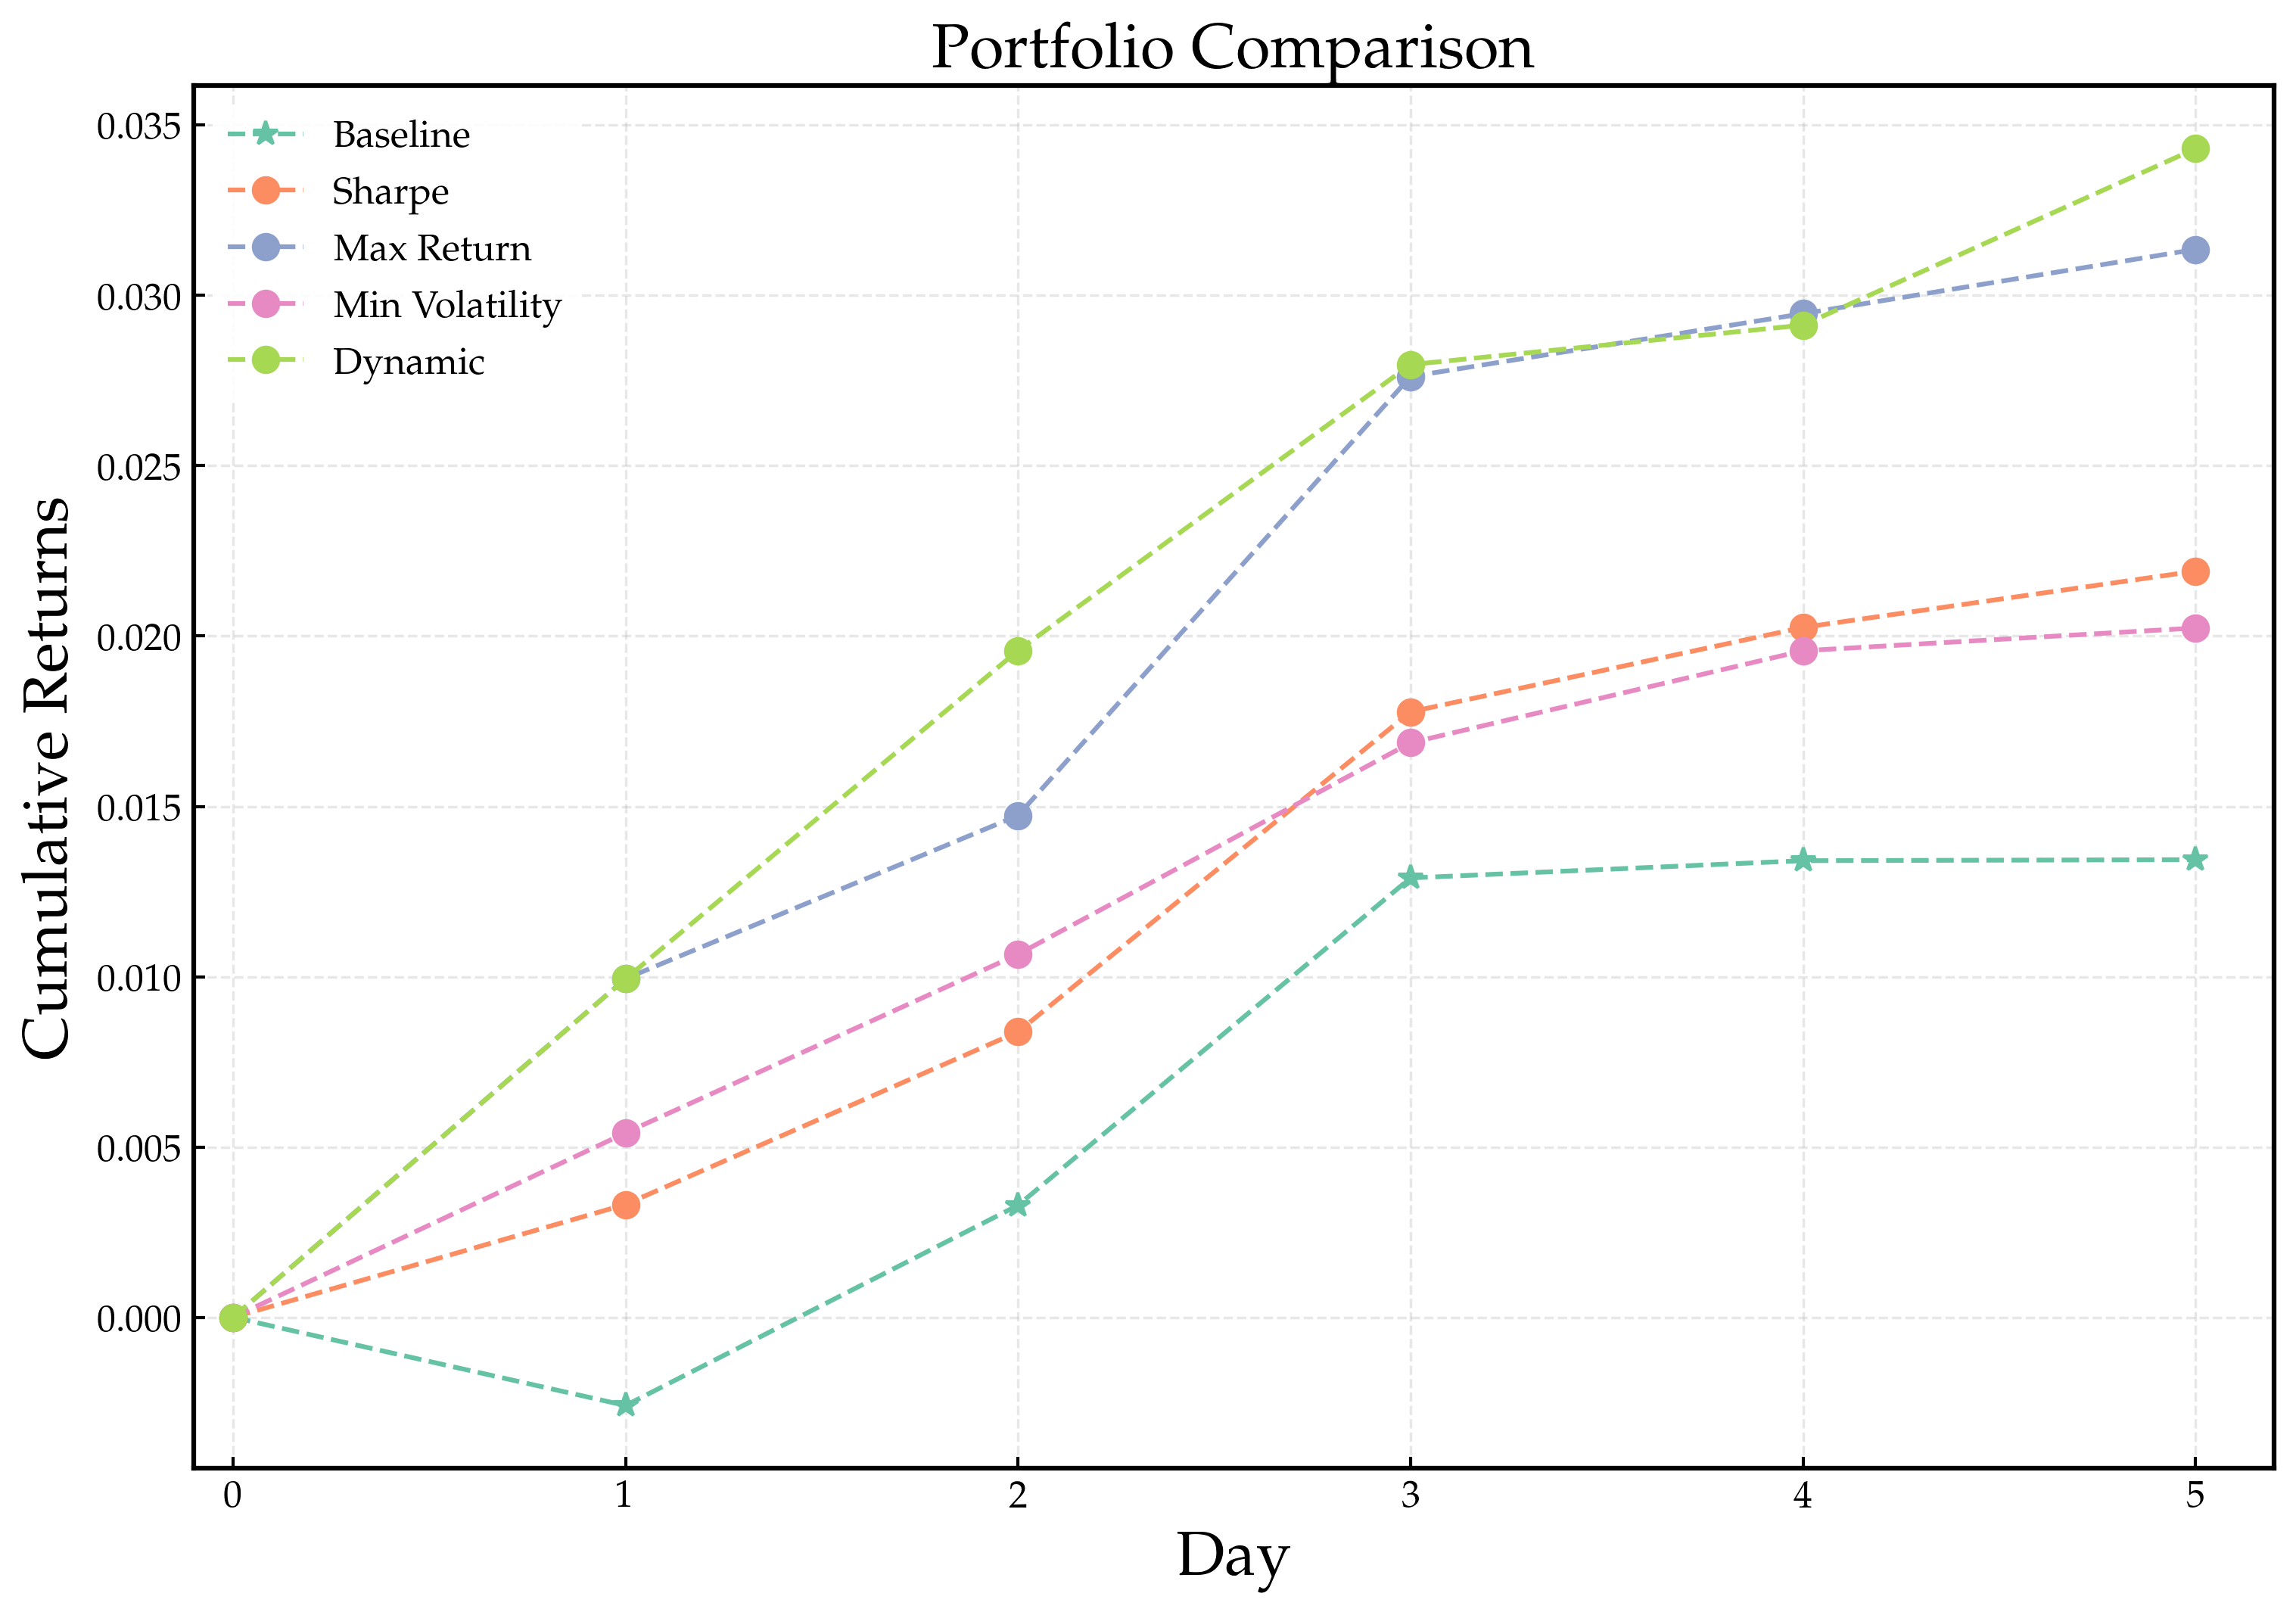
\includegraphics[width=0.6\textwidth]{figures/portfolio_comparison.png}
    \caption{Portfolio Comparison}
    \label{fig:portfolio_comparison}
\end{figure}

Risk metrics
Transaction costs impact

\begin{figure}[h]
    \centering
    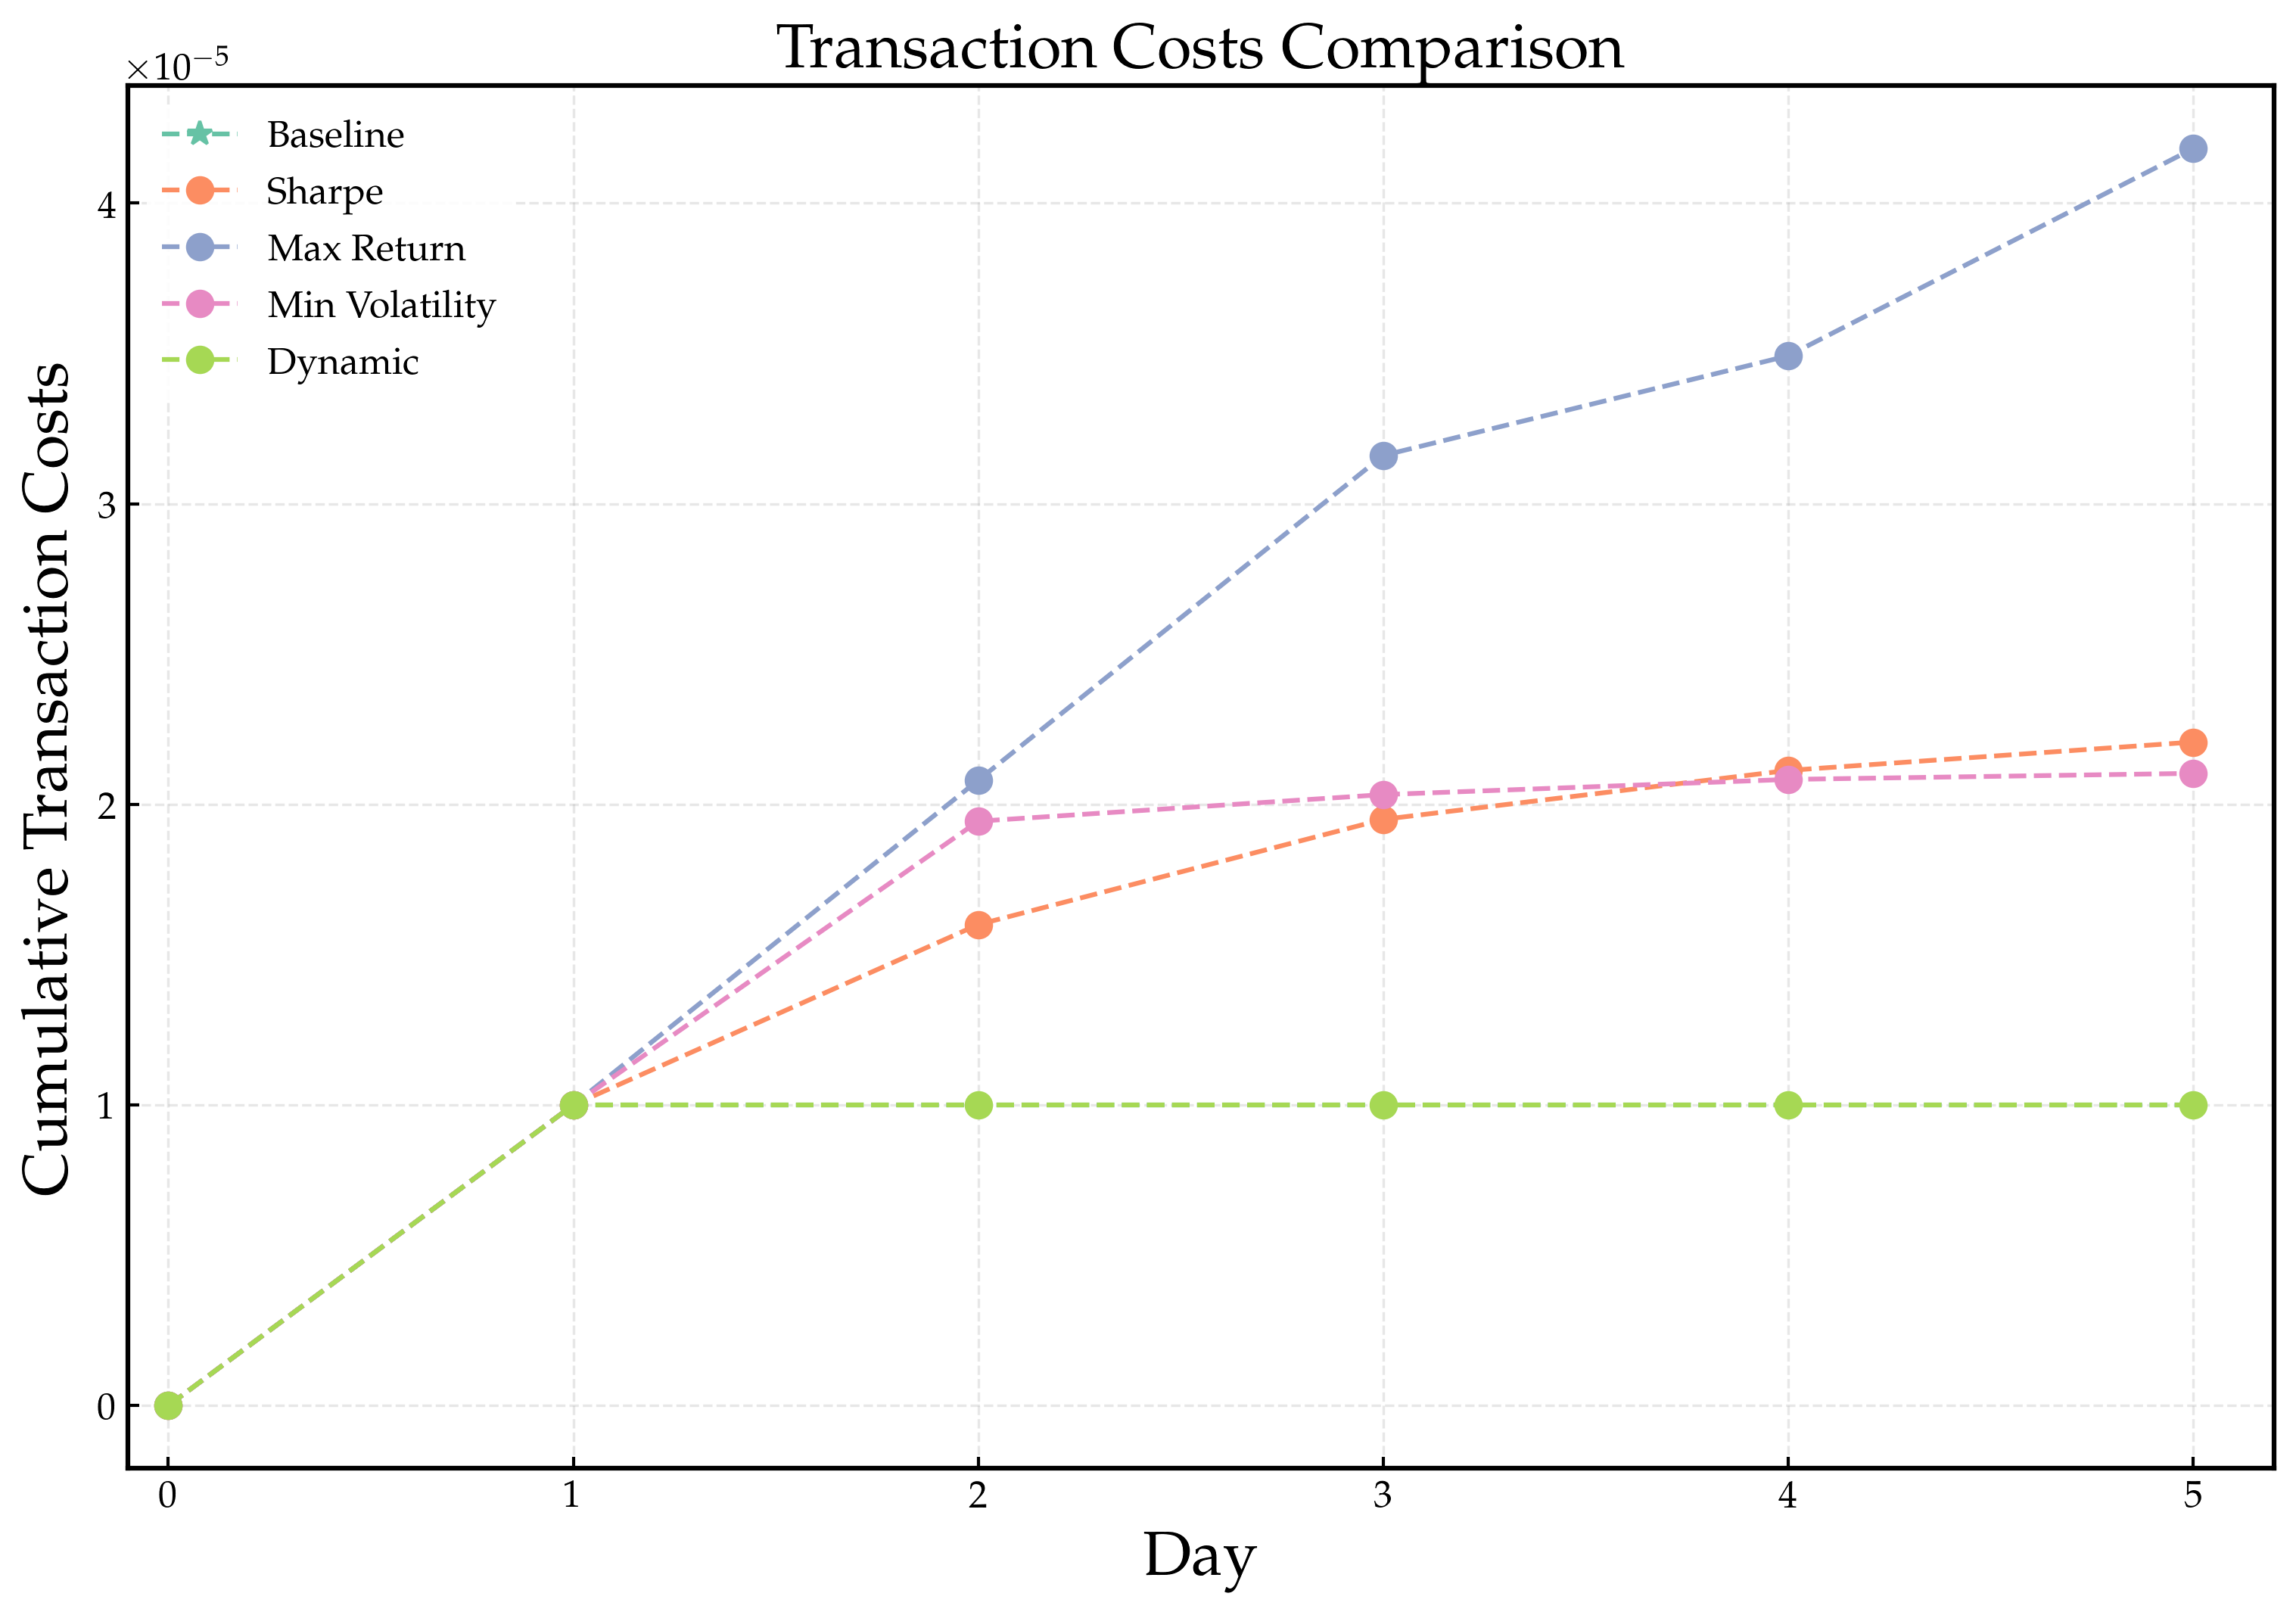
\includegraphics[width=0.6\textwidth]{figures/trx_costs_comparison.png}
    \caption{Transaction Costs Comparison}
    \label{fig:trx_costs_comparison}
\end{figure}

Strategy switching frequency analysis


Comparative Analysis:
Compare the performance of all strategies, highlighting the strengths and weaknesses of each.

\subsection{Dynamic Strategy Evaluation}
Probability threshold sensitivity
Strategy switching effectiveness
Portfolio turnover analysis
Risk-adjusted performance metrics

\subsection{Strategy Performance Calculation}

In addition to backtesting, we calculate the expected performance of the portfolio optimization strategies based on the predicted returns and the optimal weights obtained from the optimization process. This involves estimating the cumulative portfolio return and the predicted portfolio volatility, which can later be compared with the actual returns from backtesting to assess the accuracy and effectiveness of the strategies.

\subsubsection{Portfolio Class Implementation}

The \texttt{Portfolio} class is designed to manage the portfolio optimization and performance evaluation process. It integrates the optimizer, various strategies, and performance calculation methods. The key components of the class include:

\begin{itemize}
    \item \textbf{Assets}: A list of asset tickers included in the portfolio.
    \item \textbf{Asset Returns}: Historical returns of the assets.
    \item \textbf{Predicted Volatilities}: Predicted volatilities for each asset.
    \item \textbf{Optimizer}: An instance of the optimizer used for portfolio optimization.
    \item \textbf{Risk-Free Rate}: The risk-free rate used in calculations (e.g., for the Sharpe ratio).
    \item \textbf{Broker Fee}: Transaction cost rate applied to trades.
\end{itemize}

\subsubsection{Optimal Weights Calculation}

The method \texttt{get\_optimal\_weights} computes the optimal portfolio weights based on the selected strategy. It utilizes the optimizer and strategy classes to solve the optimization problem as formulated in previous sections. The optimal weights \( \mathbf{w} \) are obtained by:

\[
\mathbf{w} = \arg\min_{\mathbf{w}} \left( \text{Objective Function}(\mathbf{w}; \boldsymbol{\mu}, \Sigma) \right)
\]

subject to the relevant constraints for the chosen strategy.

\subsubsection{Strategy Evaluation Method}

The method \texttt{evaluate\_portfolio} performs the following steps to calculate the expected performance of the portfolio based on the selected strategy:

\begin{enumerate}
    \item \textbf{Initialization}: Set up initial variables, including lists to store optimal weights, predicted volatilities, covariance matrices, and daily returns.
    \item \textbf{Loop Over Time Periods}:
    \begin{enumerate}
        \item For each day \( t \) in the dataset:
        \begin{itemize}
            \item \textbf{Data Preparation}: Collect the asset returns \( \boldsymbol{\mu}_t \) and predicted volatilities \( \boldsymbol{\sigma}_t \) up to day \( t \).
            \item \textbf{Set Predictions}: Update the optimizer with the current predictions using the methods:
            \begin{itemize}
                \item \texttt{set\_predictions} for single-day predictions.
                \item \texttt{set\_cml\_log\_return} or \texttt{set\_predictions\_cml} for cumulative predictions.
            \end{itemize}
            \item \textbf{Covariance Matrix Calculation}: Compute the covariance matrix \( \Sigma_t \) using the predicted volatilities and a given correlation matrix \( \rho \):

            \[
            \Sigma_t = \text{diag}(\boldsymbol{\sigma}_t) \, \rho \, \text{diag}(\boldsymbol{\sigma}_t)
            \]

            \item \textbf{Optimal Weights Determination}: Compute the optimal weights \( \mathbf{w}_t \) for day \( t \) using the selected strategy:

            \[
            \mathbf{w}_t = \arg\min_{\mathbf{w}} \left( \text{Objective Function}(\mathbf{w}; \boldsymbol{\mu}_t, \Sigma_t) \right)
            \]

            \item \textbf{Predicted Portfolio Performance}: Calculate the predicted portfolio return \( R_{\text{portfolio}, t} \) and volatility \( \sigma_{\text{portfolio}, t} \):

            \[
            R_{\text{portfolio}, t} = \mathbf{w}_t^\top \boldsymbol{\mu}_t
            \]

            \[
            \sigma_{\text{portfolio}, t} = \sqrt{\mathbf{w}_t^\top \Sigma_t \mathbf{w}_t}
            \]
        \end{itemize}
        \item \textbf{Store Results}: Save the optimal weights and predicted volatilities for later analysis.
    \end{enumerate}
    \item \textbf{Performance Metrics Calculation}:
    \begin{itemize}
        \item \textbf{Cumulative Predicted Return}: Compute the cumulative predicted return over the time horizon:

        \[
        \text{Cumulative Predicted Return} = \prod_{t=1}^T (1 + R_{\text{portfolio}, t}) - 1
        \]

        \item \textbf{Average Predicted Volatility}: Calculate the average predicted portfolio volatility:

        \[
        \overline{\sigma}_{\text{portfolio}} = \frac{1}{T} \sum_{t=1}^T \sigma_{\text{portfolio}, t}
        \]
    \end{itemize}
\end{enumerate}

\subsubsection{Comparison with Backtesting Results}

The predicted portfolio performance metrics are compared with the actual performance obtained from backtesting to assess the accuracy and effectiveness of the optimization strategies. Key comparisons include:

\begin{itemize}
    \item \textbf{Predicted vs. Actual Returns}: Comparing the cumulative predicted return with the cumulative actual return from backtesting.
    \item \textbf{Predicted vs. Actual Volatility}: Comparing the predicted portfolio volatility with the realized volatility during backtesting.
    \item \textbf{Sharpe Ratio Analysis}: Evaluating the predicted Sharpe ratio against the actual Sharpe ratio obtained from backtesting.
\end{itemize}

\subsubsection{Implementation Notes}

\begin{itemize}
    \item \textbf{Covariance Matrix Estimation}: The covariance matrix \( \Sigma_t \) is estimated using the predicted volatilities and a given correlation matrix, capturing the relationships between assets.

    \item \textbf{Dynamic Updating}: The optimizer is updated at each time step with new predictions to reflect changes in market conditions.

    \item \textbf{Handling Log Returns}: If log returns are used, they are converted appropriately when calculating cumulative returns:

    \[
    R_{\text{portfolio}, t} = e^{R_{\text{portfolio}, t}^{\text{log}}} - 1
    \]

    \item \textbf{Multivariate Normal Distribution}: The joint distribution of asset returns is modeled using a multivariate normal distribution with mean \( \boldsymbol{\mu}_t \) and covariance \( \Sigma_t \), which is useful for probabilistic assessments in dynamic strategies.

    \item \textbf{Comparison of Strategies}: By evaluating the predicted performance of different strategies (e.g., maximum Sharpe ratio, maximum return, minimum volatility), we can identify which strategies are expected to perform better under the predicted market conditions.

    \item \textbf{Code Integration}: The \texttt{evaluate\_portfolio} method integrates with the optimizer and strategies seamlessly, ensuring that the performance calculation is consistent with the optimization process.
\end{itemize}

\subsubsection{Conclusion}

The strategy performance calculation provides essential insights into the expected performance of the portfolio optimization strategies based on predicted returns and volatilities. By comparing these predictions with actual backtested results, we can evaluate the robustness and reliability of the strategies in different market conditions. This process aids in refining the strategies and improving their practical applicability in portfolio management.



\section{Backtesting Results}
Provide detailed results from the backtesting, including cumulative returns, volatility, Sharpe ratios, and transaction costs for each strategy.

\subsection{Transaction Costs impact}

\subsection{Compared with Predicted Performance}


\subsection{Different market conditions}



\subsection{Out-of-sample performance}

\subsection{Statistical significance tests}


